\documentclass[]{article}

\usepackage{amsmath}
\usepackage[utf8]{inputenc}
\usepackage{graphicx}

\begin{document}
\author{Project 5\\
Jonas Eckhoff - Timo Greve\\ 
Max Lewerenz - Giulia Satiko Maesaka - John-Robert Wrage}
\title{Facial Emotion Recognition}
\maketitle{}

\section{Initiation Phase}
\subsection{Main goal}
\begin{itemize}
\item Develop a ``program'' for facial emotion recognition from pictures.
    \begin{itemize}
    \item Emotions: happy, sad, angry, neutral, afraid, disgusted, surprised. 
    \end{itemize}
\item Include recognition for multiple faces in a picture.
\item Include recognition from live video/webcan.
\item Achieve at least $65$\% accuracy.
\end{itemize}


\subsection{How to achieve the goal}
\begin{itemize}
\item Use deep learning for classification - Convolutional Neural Network (CNN).
\item Python Tensorflow/Keras.
\end{itemize}

\subsection{Project steps}

These first three steps constitute the \textit{Exectution Phase $1$}. The due date for Phase $1$ is the 8th of June.

\begin{itemize}
\item Training Data:
	\begin{itemize}
	\item Find first training dara for beta testing.
	\item Find better data for better/more accurate results.
	\end{itemize}

\item Programming Neural Network:
	\begin{itemize}
	\item Detect faces.
	\item Extract faces.
	\item Recognize emotion - designing a first neural network.
	\item Get first results.
	\item Optimize CNN.
	\end{itemize}
	
\item Research:
	\begin{itemize}
	\item How to optimize the neural network; find better choices for hidden layers and neurons. 
	\end{itemize}
\end{itemize}

The following step is the \textit{Execution Phase $2$}. The due date for Phase $2$ is the 15th of June.

\begin{itemize}

\item Wrapping up:
	\begin{itemize}
	\item Train final CNN with data.
	\item Final test and results.
	\item Write a ``Read me'' for the client
	\end{itemize}

\end{itemize}

The final step does not include executions of the code. The due date is the 29th of June, giving a buffer time of two weeks for unpredicted tasks or problems to be solved.

\begin{itemize}
\item Closing:
	\begin{itemize}
	\item Prepare a presentation.
	\end{itemize}

\begin{figure}
	\centering
    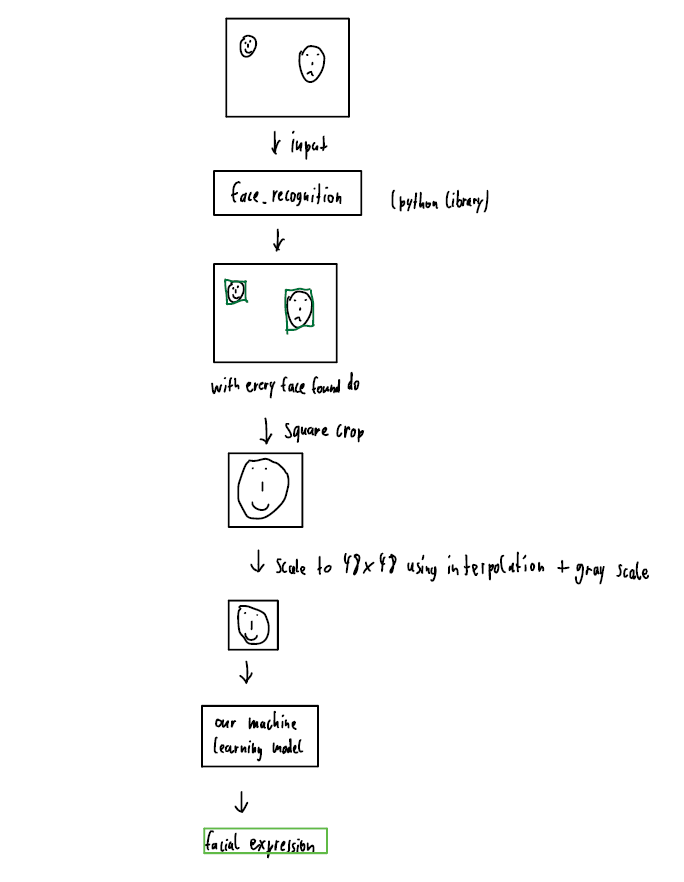
\includegraphics[height=18cm]{flow}
    \caption{Project plan}
\end{figure}

\end{itemize}

\end{document}
